\chapter{Related Work}
\section{Overview}
While during the last decades there was much progress in a field of unimodal representation, research in multimodal learning was limited by simple concatenation of unimodal features\cite{ref_survey_2015}. However, during recent years, the scientific landscape in this domain has been rapidly evolving\cite{ref_survey_baltrusaitis}. One of the triggers for it was the success of deep learning models, which have a powerful representation ability with multiple levels of abstractions. Thus they were also incorporated in multimodal learning. As Guo et al. suggested\cite{ref_survey}, we can divide all the multimodal learning approaches into three categories 1) joint representation, which aims to integrate modality-specific features into some common space 2) coordinated representation, which aims to preserve modality-specific features, while introducing a space to measure multimodal similarities  3) intermediate representation, which aims to encode features of one modal to some intermediate space, from where we later generate features of another modal.

In this chapter, we will cover available techniques to extract features from text and image modalities, overview available solutions in each type of multimodal learning, and then summarise their applicability for our problem.

\section{Unimodal Representation}
\subsection{Image}
The most popular model used in feature extraction from images are different types of Convolutional Neural Network(CNN), such as AlexNet\cite{ref_AlexNet}, VGGNet\cite{ref_VGGNet} and ResNet\cite{ref_ResNet}. When working with big datasets, it is preferable to use pre-trained version of chosen CNN. This field has tremendous development in recent years, and thus currently we already have well-defined solution for most problems.

\subsection{Text}
A popular way to extract features from the text is to encode it to vector, as is done in word2vec\cite{ref_word2vec} or Glove\cite{ref_glove} algorithms. They map words into one-hot encoded vector space of language vocabulary. Although, the common problem with those approaches is when some words are not present in vocabulary or out-of-vocabulary error. However, there are also a variety of solutions to this problem, such as character embeddings\cite{ref_char_embeddings}. 

An alternative and more powerful tool for dealing with text is recurrent neural network(RNN)\cite{ref_rnn}, which is more context-aware and can make better encoding of the n-th word, knowing what was already in a sentence. One of the most successful realizations of RNN is long short-term memory(LSTM)\cite{ref_lstm}.

\begin{figure}
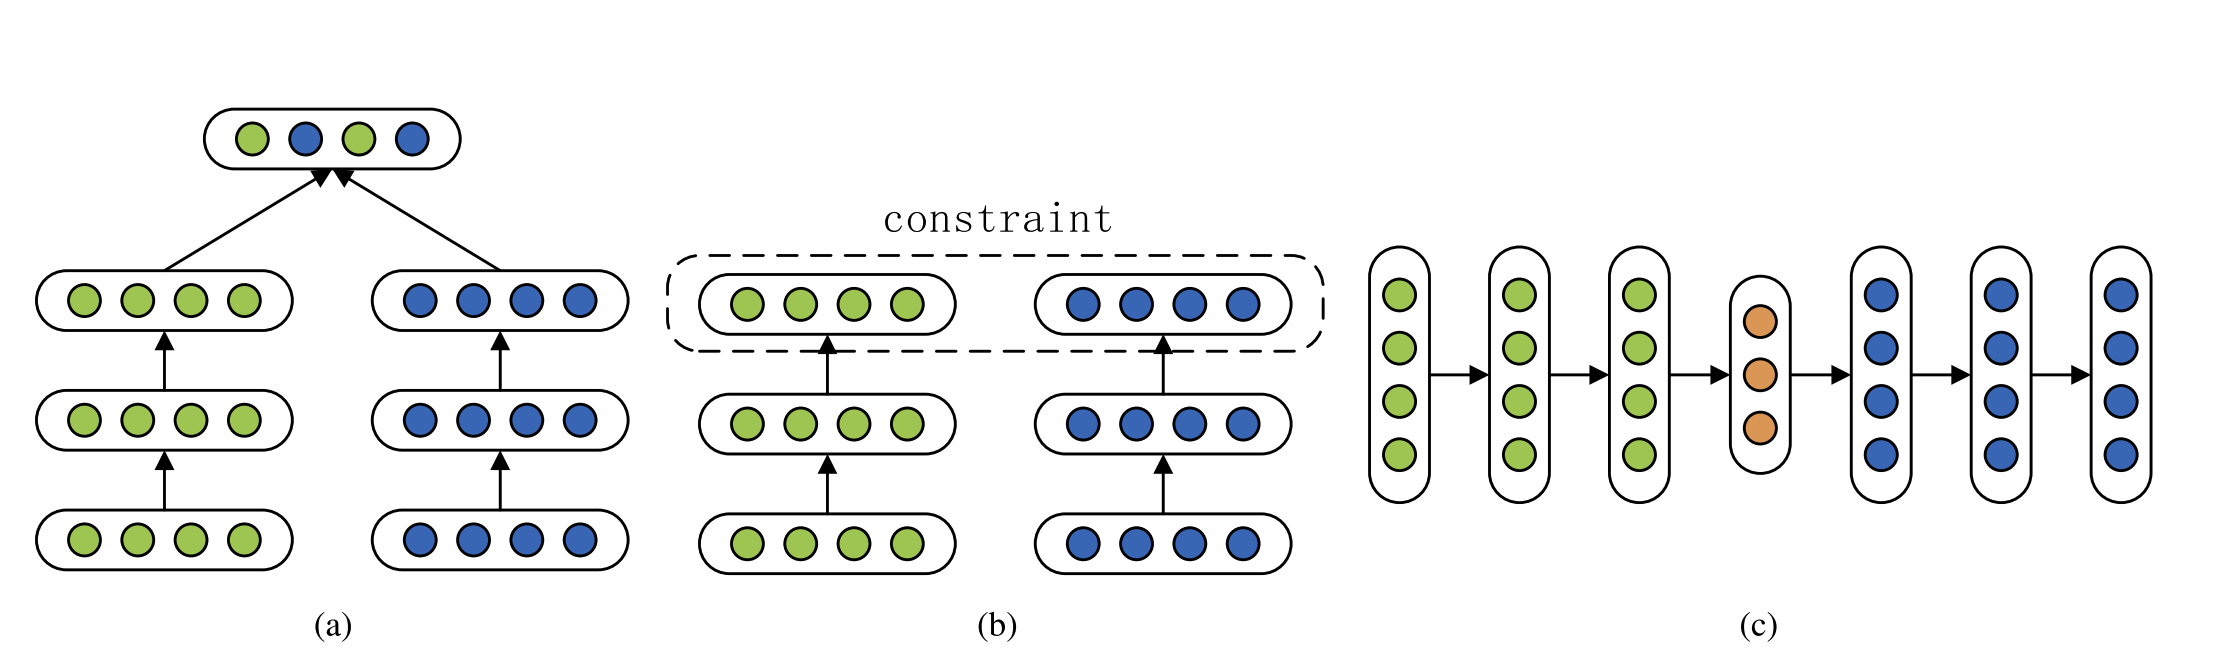
\includegraphics[width=\textwidth]{Resources/multimodal_learning_types.png}
\caption{Three types of frameworks about deep multimodal representation. (a) Joint representation aims to learn a shared semantic subspace.(b) Coordinated representation framework learns separated but coordinated representations for each modality under some constraints.
(c) intermediate representation framework translates one modality into another and keep their semantics consistent.\cite{ref_survey}} \label{fig1}
\end{figure}

\section{Joint Representation}
The main idea of joint representation is to integrate multimodal features into a single input, which we then process as some artificial unimodal input with well-known machine learning techniques. More formally, it aims to project unimodal representations into a shared semantic subspace, where the multimodal features can be fused\cite{ref_survey_baltrusaitis},  as shown in Figure \ref{fig1}(a). Up until recently, that was the primary technique in multimodal learning, where shared features were fused by concatenating them together. However, now,  the most popular choice is to use a distinct hidden layer, where modality-specific features will be combined into a single output vector.

This approach was historically the first one and is still commonly applicable in video classification\cite{ref_video_class}, event detection\cite{ref_event_detection} and visual question answering\cite{ref_visual_question_answ}. However, its main disadvantage is neglecting the fact that different modalities have not only supplementary information, that is which show the same notion from different perspectives, but also complementary information, where one modality captures the information which another cannot. For example, lips movement and audio of a speech are mostly supplementary sources, while images of some bird and audio of it singing are mostly supplementary sources. Because of that, much information gets lost in that shared space. 
% TODO: explain why in examples above one is supplementary and another complemetary

Although it has advantages of being a simple method and producing modality-invariant common space of features, it cannot be used to infer the separated representations for each modality\cite{ref_survey}. Thus methods from this category are not applicable to our problem

\section{Intermediate Representation}
Intermediate Representation models aim to encode features of one modality to some intermediate space, from which later features of another modality can be generated(or decoded), as shown on Figure \ref{fig1}(c). To prevent the intermediate space from being related only to a source modality, during encoder-decoder training we maximize, e.g., the likelihood of target sentence given source image, so that error function employs the error of decoding. Subsequently, the generated intermediate representation tends to capture the shared semantics from both modalities\cite{ref_survey}. 

Some interesting application of that model was proposed by Mor et al.\cite{ref_music_decoder}, where algorithm encodes a musical track into intermediate space, which then will be decoded by multiple decoders into a space of some specific instrument. In other words, encoder extracts instrument-invariant generic musical features, which then each decoder transforms into features of its target instrument.

The general advantage of such approach is that it is one of the best ways to generate new features in a target domain. Thus this technique is used in Image Caption\cite{ref_image_caption}, Video Description\cite{ref_video_description}, and Text to Image\cite{ref_text2image} generations. The disadvantages of that model are that 1) it can only encode one modality, 2) complexity of designing a feature generator should be taken into account\cite{ref_survey} and 3) intermediate space also extracts only shared subspace from two modalities. Moreover, because we need to query existing information rather than generate one, those methods are also not suitable for our problem solution.

\section{Coordinated Representation}
The last type of multimodal learning is a coordinated representation. Instead of learning from a joint representation, it learns from modal-specific representations separately but with a shared constraint, which is some loss function identifying cross-modal similarity/correlation. Since different modalities hold unique information about an object, that approach operates with all available knowledge. A visual explanation can be seen in Figure \ref{fig1}(b). Regarding constraint function, a commonly used option is cross-modal similarity functions, where learning objective is to preserve both inter-modality and intra-modality similarity structure. In other words, it would force cross-modal distance for elements with the same semantics be as small as possible, while with dissimilar - as big as possible. 

% TODO: specify what specifically function S can be and how it works. Note
% about copy-paste from here into solution approach
The cross-modal ranking is a widely used constrain, where the loss function is defined in the following way
\begin{equation} \label{eq_rank_loss}
\sum_i \sum_{t^-} max(0, \alpha - S(i, t) + S(i, t^-)) + \sum_t \sum_{i^-} max(0, \alpha - S(t, i) + S(t, i^-))
\end{equation}
where (i,t) is a matching image-text pair, $\alpha$ is margin, S is a similarity function, $i^-$ is mismatching pair to $t$ and vise versa. Frome et al.\cite{ref_devise} used a combination of dot-product similarity and margin rank loss to learn a visual-semantic embedding model(DeViSE) for visual recognition\cite{ref_survey}. DeViSE trains deep networks for both image and text features, and then adjust features based on above mentioned ranked loss, though in more simplified form.

Alternatively to cross-modal ranking, another widely used constraint is Euclid distance, which is also used for ensuring that similarity structure for both intra-modality and inter-modality is preserved. That is, for inter-modality, we map text and image features into low-dimensional space, where we can calculate the distance between feature vectors. The idea here is to ensure that inter-modality features of the same semantics are as close as possible\cite{ref_pan}. While for intra-modality, we want to preserve the similarity between neighborhood items, that is:
\begin{equation} \label{eq_eucl_loss}
d(m_i, m_j) + m < d(m_i, m_k), \forall m_j \in N(m_i), \forall m_k \notin N(m_i)
\end{equation}
where $m$ is data point of any modality, $m_i$ point of interest, N(m) - denotes neighborhood of m\cite{ref_wang}.
% TODO: what is m specifically in a formula? Correct it!

Besides the classical coordinated representation approach, there is a simplified version where instead of mapping both text and visual features into common space, we only map text features into visual space\cite{ref_w2vv}. In this case, we would use constant visual features, e.g. last hidden fully-connected layer of ResNet-152 pretrained on ResNet dataset\cite{ref_ResNet}. Thus we will benefit from significantly faster training time since we will only need to train one neural network for mapping text features into visual space of features. Although, the benefit comes with a cost of precision loss since we loose information specific to text modality.

So, Coordinated Representation preserves all modality-specific information. It also explicitly compares features from different modalities, thus having data from one, we can identify the closest data point from another modality. Because of those properties, it is used for cross-modal retrieval\cite{ref_wang}, retrieval-based visual description\cite{ref_socher}, and transfer knowledge across
\newline
modalities\cite{ref_pan}. Thus it can be applied for our problem of Image Recommendation for articles, and we will proceed with those methods.

\begin{figure}
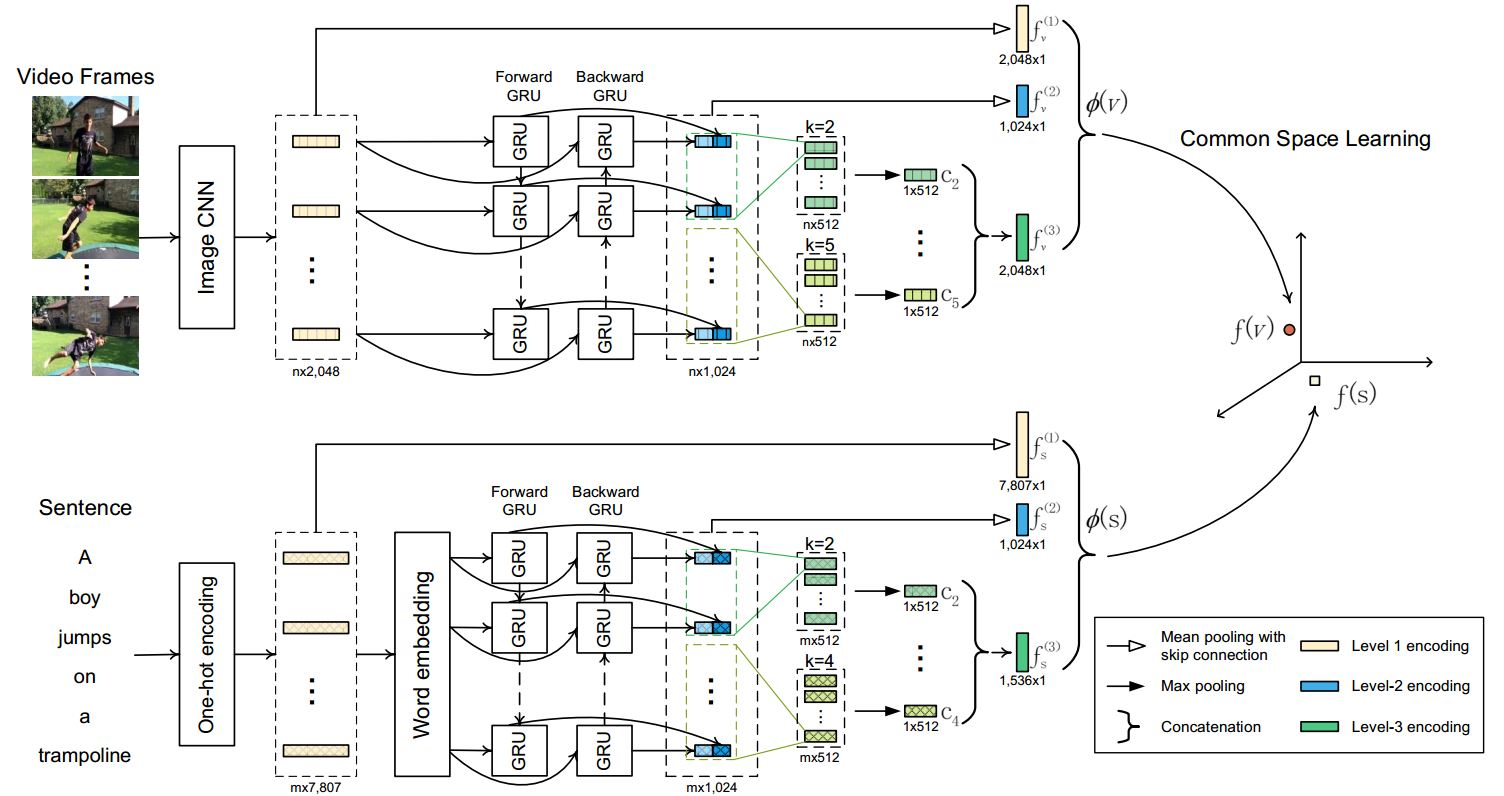
\includegraphics[width=\textwidth]{Resources/dual_encoding.jpg}
\caption{Example of Coordinated Representation learning pipeline\cite{ref_dual_encoding}} \label{fig2}
\end{figure}

\endinput